\chapter{Evaluation}
\label{ch:eval}


\section{Experimental Setup}\label{sec:experimental-setup}

We conduct our benchmarks on a Google Pixel 8 equipped with a Google Tensor G3 chip, comprising 1\,$\times$\,Cortex-X3 (2.91\,GHz), 4\,$\times$\,Cortex-A715 (2.37\,GHz), and 4\,$\times$\,Cortex-A510 (1.7\,GHz) cores, with \ac{MTE} enabled.
See \cref{tab:cores-comparison} for details on the benchmarked cores.
As of the time of writing, this is the sole commercially available device featuring \ac{MTE}.
To mitigate thermal throttling, we attach a cooling fan to the device.
Each performance test is run on each CPU type available on the Tensor G3 chip by pinning it to a single respective core.


\begin{table}[ht]
    \centering
    \small
    \caption{Comparison of the benchmarked cores.}
    \label{tab:cores-comparison}
    \begin{tabular}{l || l | l | l}
        \textbf{Spec}      & \textbf{Cortex-X3}    & \textbf{Cortex-A715} & \textbf{Cortex-A510} \\
        \hline
        Cores              & 1                     & 4                    & 4                    \\
        Pipeline           & in-order              & out-of-order         & out-of-order         \\
        Superscalar        & Yes                   & Yes                  & Yes                  \\
        Architecture       & ArmV9.2               & ArmV9.2              & ArmV9.2              \\
        Maxmimum Frequency & 2.91\,GHz             & 2.37\,GHz            & 1.7\,GHz             \\
        L1 I-Cache/D-Cache & 64\,KiB               & $32/64$\,KiB         & $32/64$\,KiB         \\
        L2 Cache           & 512\,KiB -- 1024\,KiB & 128\,KiB -- 512\,KiB & 128\,KiB -- 512\,KiB \\
        L3 Cache           & 512\,KiB -- 16\,MiB   & 512\,KiB -- 32\,Mib  & 256\,KiB -- 16\,Mib  \\
    \end{tabular}
\end{table}


\begin{table}[ht]
    \centering
    \small
    \caption{Runtime benchmarking configurations.}
    \label{tab:benchmark-variants}
    \begin{tabular}{c || c|c|c}
        \textbf{Variant} & \textbf{Pointer Width} & \textbf{Memory Safety} & \textbf{MTE Bounds Checks} \\
        \hline
        wasm32           & 32-bit                 & No                     & No                         \\
        wasm64           & 64-bit                 & No                     & No                         \\
        mem-safety       & 64-bit                 & Yes                    & No                         \\
        mte-bounds       & 64-bit                 & No                     & Yes                        \\
        combined         & 64-bit                 & Yes                    & Yes                        \\
    \end{tabular}
\end{table}

\noindent
We run the benchmarks from the PolyBench/C 3.2 suite~\cite{polybenchc}.


\section{Performance Overheads}
\label{sec:performance-overheads}

\begin{figure}[ht]
    \centering
    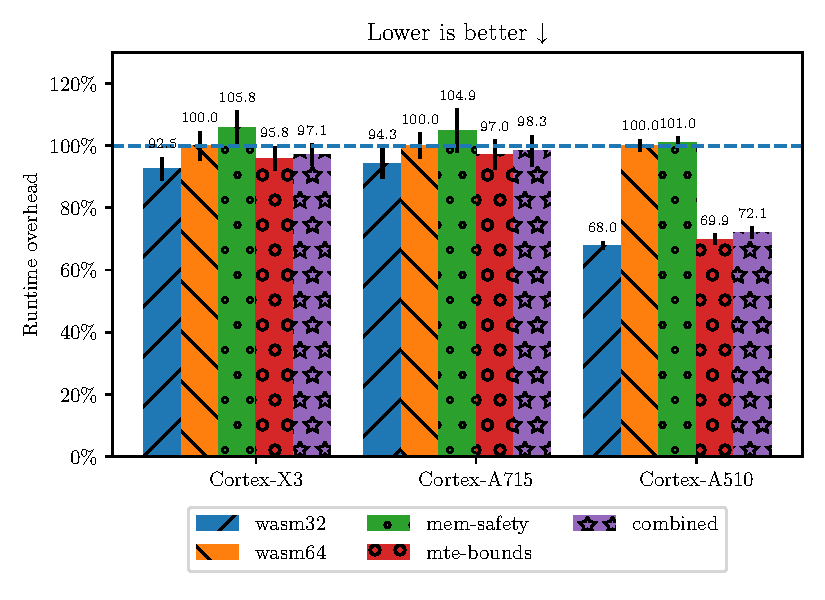
\includegraphics{plots/runtimes-all}
    \caption{PolyBench/C runtime overheads of different configurations described in \cref{tab:benchmark-variants}, normalized to wasm64.}
    \label{fig:runtime-overheads-combined}
\end{figure}

\Cref{fig:runtime-overheads-combined} illustrates the mean runtime overheads for PolyBench/C benchmarks for each CPU core available on the Tensor G3 chip.
Compared to wasm64, our memory safety extension has a mean overhead of 5.8\,\% and 4.9\,\% on the two out-of-order high-performance cores.
On the in-order Cortex-A510, we see an overhead of just 1.0\,\%.
Generally, we see that the overhead of bounds checks through the switch from wasm32 to wasm64 is lower on the out-of-order cores, as those can speculate on bounds checks, while the in-order cores cannot.
This also explains the low overhead of our memory safety extension on the in-order cores, as we spend more time doing bounds checks than on the in-order cores.

When we replace software-based bounds checks with \ac{MTE} bounds checks, we see the overhead largely disappearing.
The remaining overhead can be explained through (1) the natural overhead that enabling \ac{MTE} synchronous mode poses (see \cref{subsec:synchronous-and-asynchronous-mode}) and (2) the fact that the linear memory needs to be tagged on program startup.
This overhead is especially noticeable for short-running modules that require large amounts of linear memory.

Combining both \ac{MTE} bounds and \ac{MTE} memory safety, we see a slight increase from just \ac{MTE} bounds, which is smaller than the jump from wasm64 to memory safety.
The smaller increase is because we are not adding the \ac{MTE} overhead, as \ac{MTE} is already enabled.
The jump we see is the result of additional instructions tagging the segments.

We could decrease the overhead even further by switching to \ac{MTE} async mode, which is faster than sync mode (see \cref{subsec:synchronous-and-asynchronous-mode}).
However, this dramatically reduces the security guarantees provided by \ac{MTE}, as illegal writes and reads may become observable.
This disqualifies async \ac{MTE} for bounds checking of \ac{WASM} sandboxes, as attackers may carefully craft malicious code to escape their sandbox.
For the memory safety extension, users may decide the additional risk is worth the reduced overhead, e.g., when the memory safety extension is not used as a primary defense mechanism but as a second layer or to find bugs in the wild.


\section{Memory Overheads}\label{sec:memory-overheads}

Memory tagging incurs overhead, particularly for small allocations due to the 16-byte alignment required for \ac{MTE}.
Our measurements did not show a significant difference in maximum \ac{rss}.
This is because (1) safe allocations do not incur space overhead, and (2) for large allocations, the 16-byte alignment overhead is proportionally small.
The main overhead in \cref{fig:memory-overheads} is primarily due to the switch to wasm64, as pointer sizes are doubled.

\begin{figure*}[t]
    \centering
    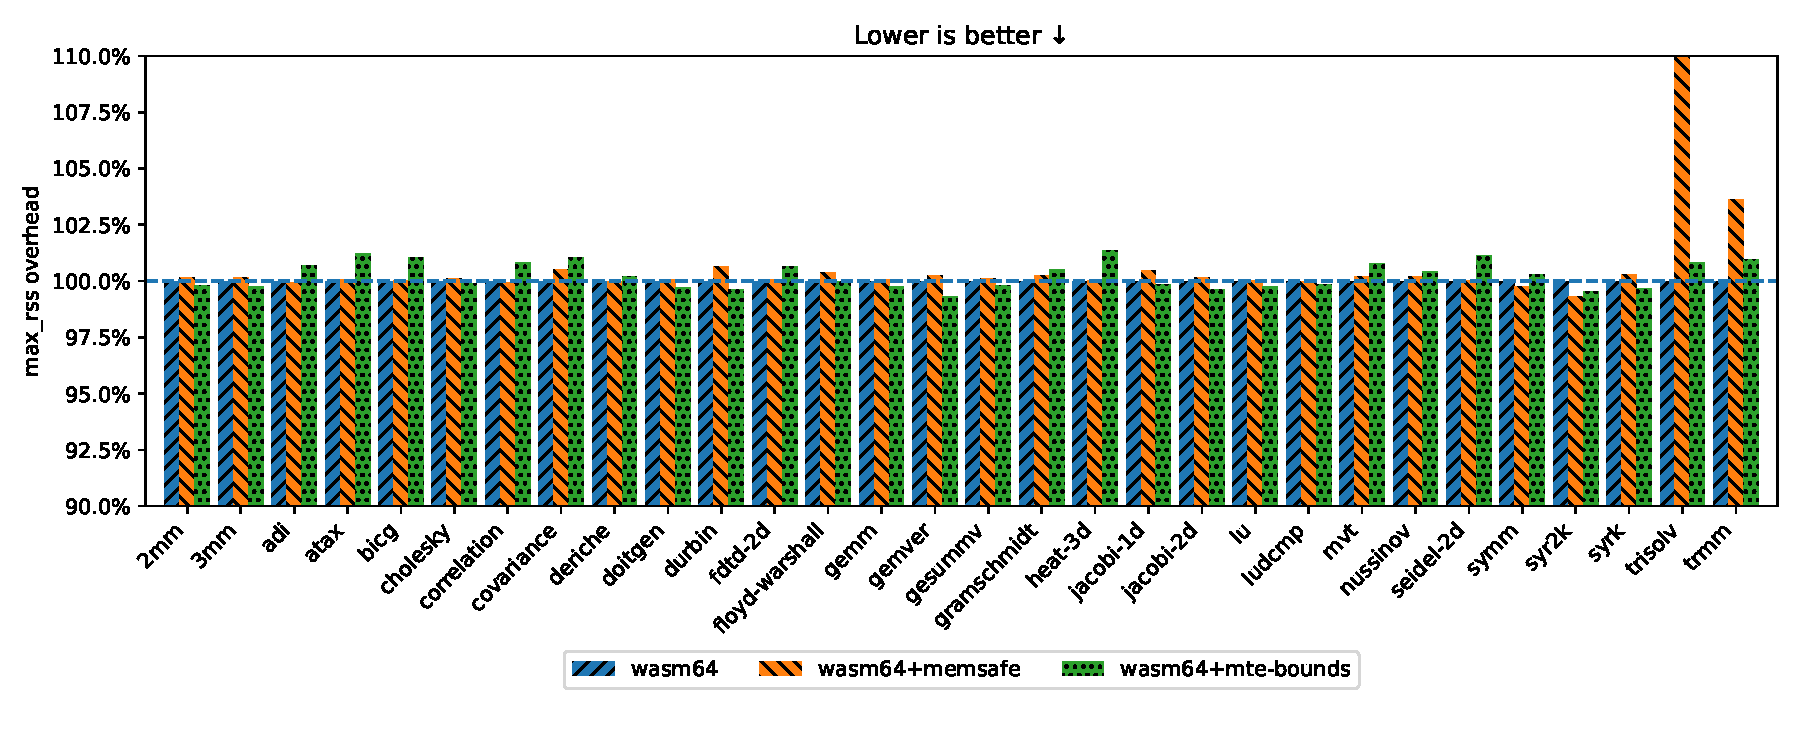
\includegraphics{plots/mem-overhead}
    \caption{PolyBench/C memory overheads of different configurations described in \cref{tab:benchmark-variants}, normalized to wasm64.}
    \label{fig:memory-overheads}
\end{figure*}


\section{Security Guarantees}\label{sec:security-guarantees}

We evaluate the security guarantees from the perspective of internal and external memory safety, as defined in \cref{sec:threat-model}.

\subsection{External Memory Safety}
\label{subsec:sec-guarantees-external-memory-safety}

Running with \ac{MTE} bounds checks, with \ac{MTE} being configured to run in synchronous mode, prevents programs from escaping their sandbox.
We prevent programs from forging tags by masking the respective tag bits before computing the effective address, as described in \cref{subsec:bounds-checks}.
Other defense mechanisms, such as structured control flow, the typed stack, and function calls through typed and checked tables, remain unchanged by our implementation.
However, we limit the number of sandboxes in one process to at most 15, which is required to assign a distinct tag to each sandbox.

Switching to async \ac{MTE} mode is not feasible to retain external memory safety, as memory accesses outside the sandbox may become observable to the \ac{WASM} module performing the illegal access and to other modules.

\subsection{Internal Memory Safety}
\label{subsec:sec-guarantees-internal-memory-safety}

Our choice to leverage \ac{MTE} allows for a low overhead, so this can be deployed in addition to testing using other mechanisms, such as \ac{ASAN}.
However, our approach does not provide complete memory safety for internal memory safety, as \ac{MTE} provides a limited number of tags and should be used as a secondary, not primary, defense mechanism to harden applications in the wild.
A tag collision means two memory regions could accidentally share the same tag, potentially leading to a missed security violation.
For example, if a buffer overflow writes slightly beyond its intended bounds, but the adjacent memory has the same tag, \ac{MTE} cannot detect the issue.

We can calculate the probability for a tag collision for $k=2$ random tags according to \cref{fig:tag-collision}, with $n=16$ available tags for \ac{MTE} bounds disabled (\cref{fig:tag-collision-16}) and $n=8$ for bounds enabled (\cref{fig:tag-collision-8}), as we reserve one bit for the bounds checking mechanism.

\begin{figure}[h]
    \centering
    \begin{subfigure}[T]{0.45\textwidth}
        \centering
        \begin{align*}
            V_{nr} &= \frac{n!}{(n - k)!} = 240 \\
            V_t &= n^k = 256 \\
            P(\text{c}) &= 1 - \frac{V_{nr}}{V_t} = 6.25\%
        \end{align*}
        \caption{Probability of a tag collision with $n=16$ and $k=2$.}
        \label{fig:tag-collision-16}
    \end{subfigure}
    \hfill
    \begin{subfigure}[T]{0.45\textwidth}
        \centering
        \begin{align*}
            V_{nr} &= \frac{n!}{(n - k)!} = 56 \\
            V_t &= n^k = 64 \\
            P(\text{c}) &= 1 - \frac{V_{nr}}{V_t} = 12.5\%
        \end{align*}
        \caption{Probability of a tag collision with $n=8$ and $k=2$.}
        \label{fig:tag-collision-8}
    \end{subfigure}
    \caption{Probabilities of tag collisions for random tags.}
    \label{fig:tag-collision}
\end{figure}

However, we ensure that adjacent allocations are always tagged with distinct tags and that memory is tagged with a new tag when it is freed, thus ensuring that spatial errors up to 16\,bytes and temporal errors until the subsequent allocation of a chunk of memory are always caught.


\section{MTE Performance evaluation}
\label{sec:mte-performance-evaluation}

We evaluated the performance of different characteristics of \ac{MTE} as implemented on the Tensor G3 chip.
All the programs used to measure results in this section are implemented in Rust and available on GitHub\footnote{\url{https://github.com/martin-fink/mte-stg-bench}}.
As our benchmarking library, we used criterion\footnote{\url{https://github.com/bheisler/criterion.rs}}.
After each benchmarking run, we let the device cool down for 30\,seconds to prevent throttling.
Additionally, we measure instruction throughput and latencies on all CPU cores.

\subsection{Instruction Latencies and Throughput}\label{subsec:instruction-latencies-and-throughput}

We evaluate instruction latencies and throughput in microbenchmarks executing 100,000,000 iterations of 100 instructions to minimize the effect of the looping code.
We use simpleperf\footnote{\url{https://android.googlesource.com/platform/system/extras/+/master/simpleperf/doc/README.md}} to measure CPU cycles of our benchmarking program\footnote{\url{https://github.com/martin-fink/mte-inst-cycles}}.
For each instruction, we measure three variants: (1) the baseline, which includes the startup, setup, and teardown of the benchmark, where no actual instructions are executed, (2) the latency test, where we measure instructions with data dependencies between them, and (3) the throughput test, where we measure instructions with no data dependencies.
We see the cycles and micro-ops per instruction in \cref{tab:instruction-latencies}.

We can make a few interesting observations:
\begin{itemize}
    \item For the set-tag instructions, Cortex-X3 has double the latency and half the throughput compared to Cortex-A720.
    \item On Cortex-A510, \texttt{st2g} has double the latency and half the throughput of \texttt{stg}, while also being the only one with two micro-ops per instruction.
    This leads us to believe that this instruction performs the same micro-op as \texttt{stg}, but for two tag granules, while the operation is optimized on the other cores.
    \item Loading tags has a higher latency and lower or equal throughput than storing tags, except for the Cortex-X3.
    \item As expected, we found latency-bound instructions to perform as many or more cycles per instruction compared to throughput-bound instructions.
\end{itemize}

\newcolumntype{C}{>{\centering\arraybackslash}p{2em}}
\begin{table}[h]
    \centering
    \small
    \caption{MTE cycles per instruction when latency- and throughput-bound (lower is better), and micro-ops per instruction.}
    \label{tab:instruction-latencies}
    \begin{tabular}{c || C | C | C | C | C | C | C | C | C }
        \multirow{2}{*}{\textbf{Variant}} & \multicolumn{3}{c|}{\textbf{Cortex-X3}} & \multicolumn{3}{c|}{\textbf{Cortex-A720}} & \multicolumn{3}{c}{\textbf{Cortex-A510}} \\
        & Lat & Tp   & $\mu$ops & Lat & Tp  & $\mu$ops & Lat & Tp & $\mu$ops \\
        \hline
        \texttt{irg}  & 2   & 0.75 & 3        & 2   & 1   & 3        & 3   & 2  & 1        \\
        \texttt{ldg}  & 1   & 1    & 2        & 1.5 & 1   & 2        & 4   & 4  & 1        \\
        \texttt{stg}  & 1   & 1    & 2        & 0.5 & 0.5 & 2        & 1.5 & 1  & 1        \\
        \texttt{st2g} & 1   & 1    & 2        & 0.5 & 0.5 & 2        & 3   & 2  & 2        \\
        \texttt{stgp} & 1   & 1    & 2        & 0.5 & 0.5 & 2        & 1.5 & 1  & 1        \\
        \texttt{stzg} & 1   & 1    & 2        & 0.5 & 0.5 & 2        & 1.5 & 1  & 1        \\
    \end{tabular}
\end{table}

\subsection{Tagging Primitives}
\label{subsec:tagging-primitives}

We evaluated the performance of the different types of instructions to set the tag for a memory granule available in EL0 (user space) with the combinations described in \cref{tab:stg-instructions}.
Here, instruction refers to the instruction used to set the tag, and granule size refers to the amount of memory being tagged with a single instruction.
The instructions \texttt{stzg} and \texttt{stgp} implicitly set the granule to zero, while we have to use an explicit memset for other instructions.

\begin{table}[h]
    \centering
    \small
    \caption{MTE benchmarking variants.}
    \label{tab:stg-instructions}
    \begin{tabular}{c || c | c | c | c }
        \textbf{Variant} & \textbf{Instruction} & \textbf{Granule size} & \textbf{Implicit zero} & \textbf{memset} \\
        \hline
        memset           & -                    & -                     & No                     & Yes             \\
        stg              & \texttt{stg}         & 16                    & No                     & No              \\
        st2g             & \texttt{st2g}        & 32                    & No                     & No              \\
        stgp             & \texttt{stgp}        & 16                    & Yes                    & No              \\
        stzg             & \texttt{stzg}        & 16                    & Yes                    & No              \\
        stg+memset       & \texttt{stg}         & 16                    & No                     & Yes             \\
        st2g+memset      & \texttt{st2g}        & 32                    & No                     & Yes             \\
    \end{tabular}
\end{table}

We run the benchmark on our testbed (see \cref{sec:experimental-setup}) tagging a 128\,MiB memory region.
Before each run, we request a fresh piece of memory with \texttt{mmap} and run the specified configuration to prevent interference through already-filled caches.

\begin{figure}[h]
    \centering
    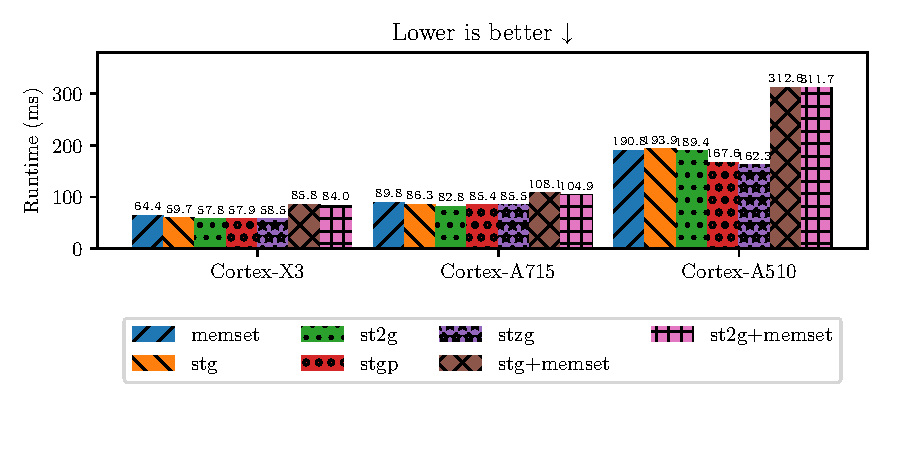
\includegraphics{plots/stg}
    \caption{Performance results of the benchmarking variants from \cref{tab:stg-instructions} on 128\,MiB of memory.}
    \label{fig:stg-performance}
\end{figure}

We perform all runs on each type of CPU core on the Pixel 8 and illustrate the results in \cref{fig:stg-performance}.
As expected, the instructions implicitly setting the memory to zero are faster than tagging and then zeroing using an explicit memset.
Both \texttt{stzg} and \texttt{stgp} are only slightly slower than a raw memset, as their memory accesses do not need to perform tag checks~\cite{ARMA2024Arch64}.

Contrary to our expectations, \texttt{st2g} is only marginally faster than \texttt{stg}.
This finding contradicts the data presented in \cref{subsec:instruction-latencies-and-throughput}, where operations are performed with pre-filled data caches.
In these benchmarks, we specifically measure wall clock time, not processor cycles, to evaluate performance when tagging a large region of memory immediately after requesting it from the operating system.
This approach involves requesting a fresh segment of memory before each execution.
The Cortex-X3 achieves shorter execution times than the Cortex-A720, despite us measuring lower instructions executed per cycle, due to its higher clock speed.

\subsection{Synchronous and Asynchronous Mode}
\label{subsec:synchronous-and-asynchronous-mode}

We evaluate the performance of sequential memory accesses with \ac{MTE} disabled and enabled using synchronous mode and asynchronous mode on each type of CPU core on the Pixel 8.
This represents the raw overhead of enabling \ac{MTE} without additional instructions.
In \cref{fig:sync-async-performance}, we see that with synchronous mode, \texttt{memset} is 11.5\%, 8.9\%, and 13.2\% slower on the respective cores compared to the baseline with \ac{MTE} disabled.
Asynchronous mode is closer to the baseline with an overhead of 0.9\%, 3.7\%, and 6.1\% respectively.

\begin{figure}[h]
    \centering
    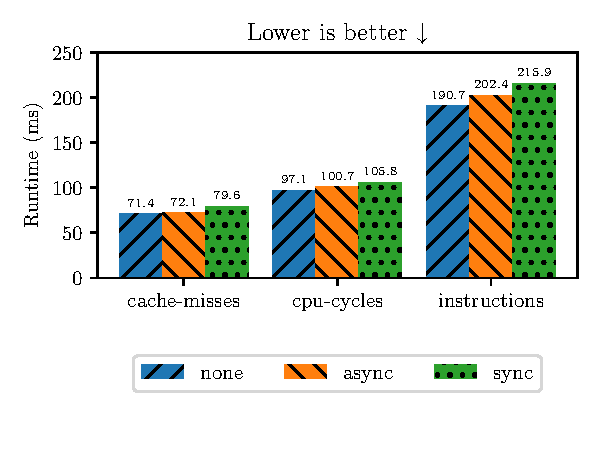
\includegraphics{plots/sync-async}
    \caption{Runtime of \texttt{memset} on 128\,MiB of memory using different \ac{MTE} modes.}
    \label{fig:sync-async-performance}
\end{figure}

\subsection{Migrating Tagged Memory}
\label{subsec:migrating-tagged-memory}

Migrating tagged memory involves the coordinated transfer of both data and its associated tags.
In \cref{fig:migrate-performance}, we analyze the performance of two migration strategies.

\begin{enumerate}
    \item Baseline (\texttt{memcpy} with \ac{MTE}): This baseline establishes the cost of a standard memory copy operation with \ac{MTE} enabled.
    \item \ac{MTE} Disable/Re-enable: Disabling \ac{MTE}, copying data with \texttt{memcpy}, transferring tags, and re-enabling \ac{MTE}.
    This method temporarily compromises memory safety during the transfer if other threads rely on \ac{MTE} being active during this approach.
    \item Iterative Copying: Copying tags and data in 16\,byte granules allows copying tags and data simultaneously while keeping \ac{MTE} active for other threads.
\end{enumerate}

\noindent
Approach 3 is slightly slower than approach 2 on the Cortex-X3 but faster on the other cores.

\begin{figure}[h]
    \centering
    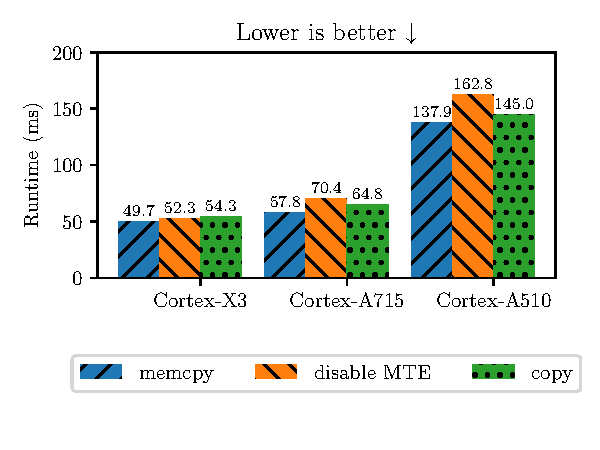
\includegraphics{plots/migrate}
    \caption{Runtime comparison of strategies for moving 128 MiB of memory and tags between regions.}
    \label{fig:migrate-performance}
\end{figure}
